\documentclass[11pt]{scrartcl}
\usepackage{graphicx}
\graphicspath{{./}}
\usepackage[sexy]{evan}
\usepackage[normalem]{ulem}
\usepackage{hyperref}
\usepackage{mathtools}
\hypersetup{
    colorlinks=true,
    linkcolor=blue,
    filecolor=magenta,      
    urlcolor=cyan,
    pdfpagemode=FullScreen,
    }
\usepackage[most]{tcolorbox}
\renewcommand{\dangle}{\measuredangle}

\renewcommand{\baselinestretch}{1.5}

\addtolength{\oddsidemargin}{-0.4in}
\addtolength{\evensidemargin}{-0.4in}
\addtolength{\textwidth}{0.8in}
% \addtolength{\topmargin}{-0.2in}
% \addtolength{\textheight}{1in} 


\setlength{\parindent}{0pt}

\usepackage{pgfplots}
\pgfplotsset{compat=1.15}
\usepackage{mathrsfs}
\usetikzlibrary{arrows}

\title{Extra Problems version 1.0}
\author{Compiled by Azzam Labib Hakim}
\date{Last Updated \today}

\begin{document}
\maketitle

\begin{enumerate}
    \item How many two-digit prime numbers with repeated digits are there?

    \item  12 bottles of milk contain 4 litres of milk. How many litres of milk do 45 bottles of milk contain?

    

    \item  How many terms are there in the arithmetic sequence '4, 7, 10, \ldots, 58, 61'?

    \item  Fritzy had some dumpling. After he ate 2 less than a half of the dumpling, 42 dumpling were left. How many dumpling did Fritzy have at the beginning?

    

    \item  Calculate the following expression.
    $$11 \times 13 - 17 \div 7 - 13 \times 8 +24 \div 7.$$

    \item  There are 3 red, 4 yellow, 5 blue and 6 green marbles in a bag. At least how many marbles have to be picked up to ensure that 3 marbles of different colours are picked up?

    

    \item  The sides of each small grey square are 3 centimetres long in the following figure. How many centimetres is the perimeter of the shaded area?
    \begin{figure}[h]
        \centering
        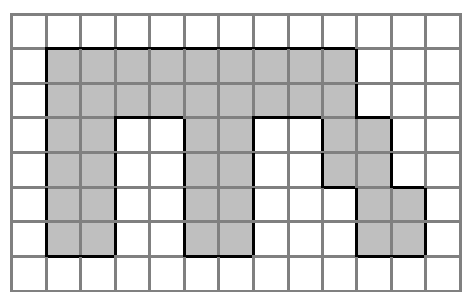
\includegraphics[width=0.4\textwidth]{StarGen/0Figure/perimeter-weird.png}
    \end{figure}

    \item  Find the remainder when $2763497219$ is divided by 9.


    \item Find the value of the following expression.
    $$(1-101) \times (3-99) \times (5-97) \times (7-95) \times \ldots \times (97-5) \times (99-3) \times (101-1).$$
    
    \item  A basketball team has five players with an average height of 185 centimetres. The average height of a point guard, shooting guard and small forward is 176 centimetres. The average height of a small forward, power forward and centre is 193 centimetres. How many centimetres high is the small forward in this basketball team?

    

    \item  It is known that the 6 apple and 8 breads cost 96 dollars in total. 1 bread is 1 dollar more expensive than 2 apple. How much does 1 apple cost in dollars?

    \item  Find the value of the following expression.
    $$214+208+202+\dots+16+10.$$

    

    \item  Among the four-digit numbers which are divisible by 12 and 18, and have non-repeated digits, what is the biggest?

    \item  If a rectangle which is 3 centimetres long and 2 centimetres wide and a rectangle which is 2 centimetres long and 3 centimetres wide are treated as the same rectangle, how many kinds of rectangles with an area of 72 square centimetres whose length and width are both integers in centimetres are there?

    

    \item  Among the 2023 natural numbers from 1 to 2024, at least how many numbers have to be picked at random so that there must be two numbers whose sum is 2024?

    \item  A 7-digit number $\overline{A1234A4}$ is divisible by 12. find the sum of possibilites of $A$.


    \item In following figure, all the angles given in the following figure are straight angles. Find the area of the figure.
    \begin{figure}[h]
        \centering
        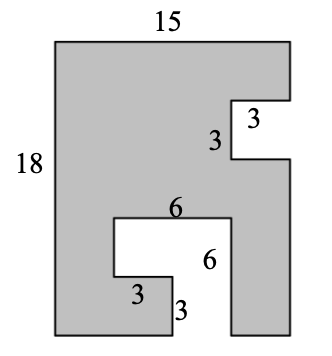
\includegraphics[width=0.4\textwidth]{StarGen/0Figure/nazi-area.png}
    \end{figure}
    
    \item  What is the 1000th term in the sequence '1, 1, 2, 1, 2, 3, 1, 2, 3, 4, 1, \ldots'?

    

    \item  A spider has 8 legs but no wings; A dragonfly 6 legs and 2 pairs of wings; A Cicadas 6 legs and 1 pair of wings. Now there are 27 insects of these three kinds. They have 180 legs and 25 pairs of wings in total. How many cicadas are there?
    
    \item  There is a book with 359 pages. Each page has a page number: 1, 2, 3, \ldots, 358, 359. How many ‘3’s are used in total for the page numbers of this book? 

    \item Find the sum of all positive factors of 42.
     \item 42 trees are planted along a road from one end to another on both sides. Every two adjacent trees are 8 metres apart. How long is the road in metres?
     \item The number $202431122024311220243112\ldots$ is written on and on. What is the $90^{th}$ digit?
     \item Evaluate the value of $3 \times (2024^2 - 2^2) \div (2022 \times 2026)$.
     \item Find the remainder when $202420242024\ldots2024$ (with 2024 "2024"'s) is divided by 9. 
     \item The ages of Mickey and Chesney add up to 95. The age of Mickey is 25 more than 4 times that of Chesney. Find the age of Mickey.
     \item Find the perimeter of the figure if all angles in the figure are right angles. 
    \begin{figure}[h]
        \centering
        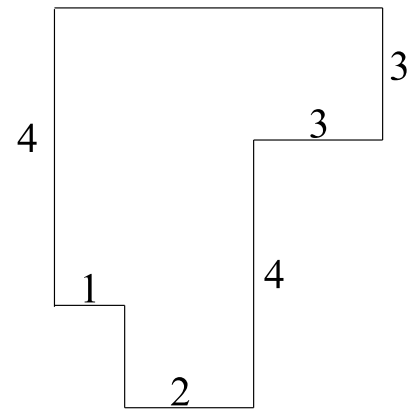
\includegraphics[width=0.4\textwidth]{StarGen/0Figure/perim.png}
    \end{figure}
     \item 6 different three-digit numbers can be formed using the digits "3", "6" and "8". Find the sum of these 6 three-digit numbers.

    \item Among the 36 natural numbers from 1 to 36, at least how many numbers have to be picked so that there must be 2 numbers whose difference is 18?
    
     \item Define the operation symbol $\oplus$ following this pattern:
    \begin{align*}
    1 \oplus 5 &= 1 - 2 + 3 - 4 + 5\\
    3 \oplus 8 &= 3 - 4 + 5 - 6 + 7 - 8\\
    5 \oplus 9 &= 5 - 6 + 7 - 8 + 9\\
    \dots& \text{(and so on ...)}
    \end{align*}
    Find the value of $(5 \oplus 10) - (4 \oplus 9).$
    
     \item Ronny runs after Sunny at a speed of 25 km/h. In the beginning, Sunny is 3 km ahead of Ronny. If Ronny manages to meet Sunny 12 minutes later, how many kilometres does Sunny run each hour?
    
     \item Define $F(a)$ as $3 \times a+1$. Find the value of $n$ if $F(F(n))=40$.
    
     \item 5 bags of rice, 6 bags of soybeans and 9 bags of red beans weigh 60 kilograms, while 17 bags of rice, 18 bags of soybean and 27 bags of red beans weigh 200 kilograms. So how many kilograms does 1 bag of rice weigh?
    
     \item There are two positive integers. Their sum is 143 and their product is 1080. Find the greater number among these two numbers.
    
     \item The four members in Mandy's family have their ages add up to 99. Her brother is 8 years younger than Mandy. Dad is 3 years older than Mum. 10 years ago, the family ages added up to 65. How old is Mum this year?
    
     \item Evaluate $20^2-18^2+16^2-14^2+\dots+4^2-2^2$.

    \item The larger rectangle in the figure is formed by 5 identical smaller rectangles. If the perimeter of the larger rectangle is $52$cm. Find the perimeter of a small rectangle. 
    \begin{figure}[h]
        \centering
        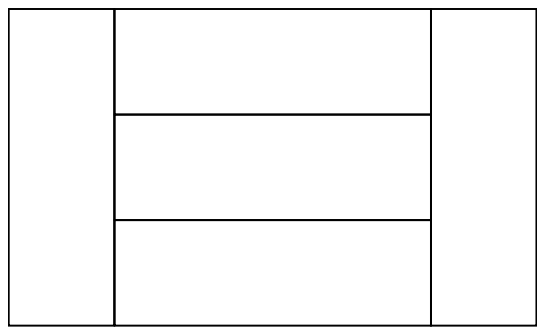
\includegraphics[width=0.4\textwidth]{StarGen/0Figure/5rect2.png}
    \end{figure}
    
     \item A Hacker enters the password "394052186" when he comes to a system of computers. The system says they have swapped two of the numbers. How many passwords at most does the Hacker need to enter more?

     \item There are 55 cards. "1" is written on 1 card, "2" on 2 cards, "3" on 3 cards, \ldots, "10" on 10 cards. Now several cards are picked so that the sum of the numbers on all cards is 312. How many cards can be picked at most?
    
    \item The figure shows some numbered squares. If squares are to be tiled up to 2024 following the pattern, find the number in the square which is just above 127. 
    \begin{figure}[h]
        \centering
        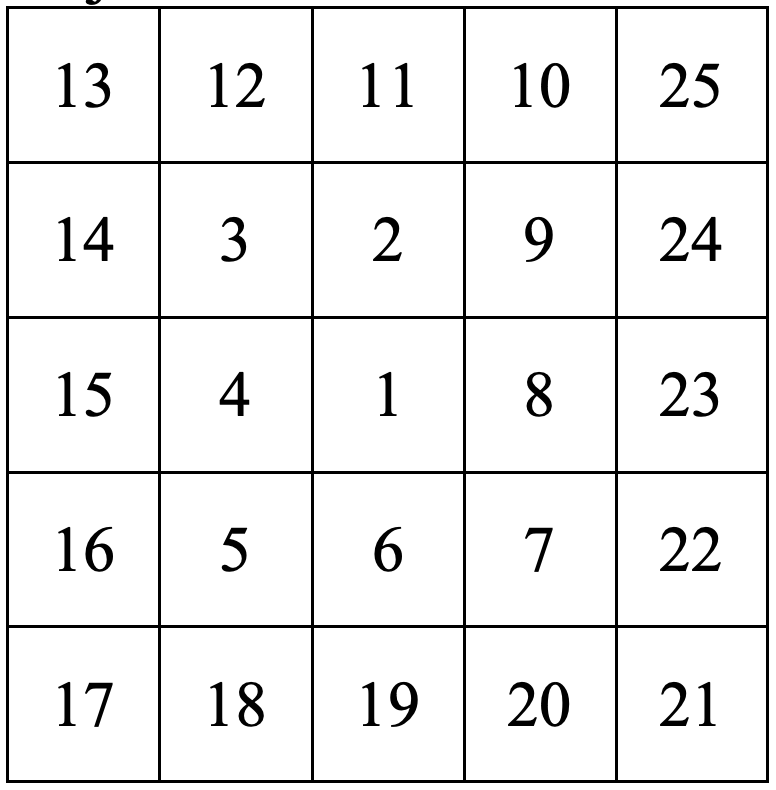
\includegraphics[width=0.4\textwidth]{StarGen/0Figure/square-siput.png}
    \end{figure}
\end{enumerate}

\end{document}